% Instructions to change to html version:
% Comment out:
%  minipage, multicols,columnbreak, mathbf, hrule
% Replace all: \begin{minipage}% %%\end{minipage} %%%%\begin{mulicols}  %%%%\end{mulicols}  %%%\columnbreak % %%%\begin{framed} %%%%\end{framed} %%%\hrule
% Search for \mathbf \mathcal
% Replace \\] with \[ and \) with \(
% Enclose graphics in figure environments and add captions
% Re-tag \df environments as sections, subsections, etc.
% Command Line Code to Create html version:
%First: pdflatex -shell-escape filename.tex                                   
%Second, for each figure: inkscape "filename-figure1.pdf" -o "filename-figure1.png"
% Third: htlatex filename.tex "ht5mjlatex.cfg, charset=utf-8" " -cunihtf -utf8"


\documentclass[10pt]{article}

%\usepackage{tikz, pgf,pgfplots,wasysym,array}
%\usepackage{wasysym}

\usepackage{amsmath,amssymb}

\ifdefined\HCode
  \def\pgfsysdriver{pgfsys-tex4ht-updated.def}
\fi 
%\ifdefined\HCode
%  \def\pgfsysdriver{pgfsys-dvisvgm4ht.def}
%\fi 
\usepackage{tikz}
\usetikzlibrary{calc,decorations.markings,arrows}
\usepackage{pgfplots}

\pgfplotsset{compat=1.12}
\usepackage{myexternalize}
%\usetikzlibrary{calc,decorations.markings,arrows}
\usepackage{framed}
\usepackage[none]{hyphenat}

\input{../../../common/1336_header_test.tex}

\begin{document}

\everymath{\displaystyle}

\renewcommand{\myTitle}{MATH 2330: Multivariable Calculus}

\renewcommand{\mySubTitle}{Section 5.2: Double Integrals over General Regions}
%~\hfill Name: \underline{~~~~~~~~~~~~~~~~~~~~~~~~~~~~~~~~~~~~~~~~~~~~~~~}

\lectTitle{\vspace*{-.5in}\myTitle}{\vspace*{.1in}\mySubTitle \vspace*{-.25in}}

\setlength{\columnseprule}{0.4pt}
\setlength{\columnsep}{3em}

%\hspace*{-.8in}\begin{minipage}{1.25\textwidth}
%\begin{framed}

%\begin{multicols}{2}

\section*{Vertically Simple or Type I Regions:}


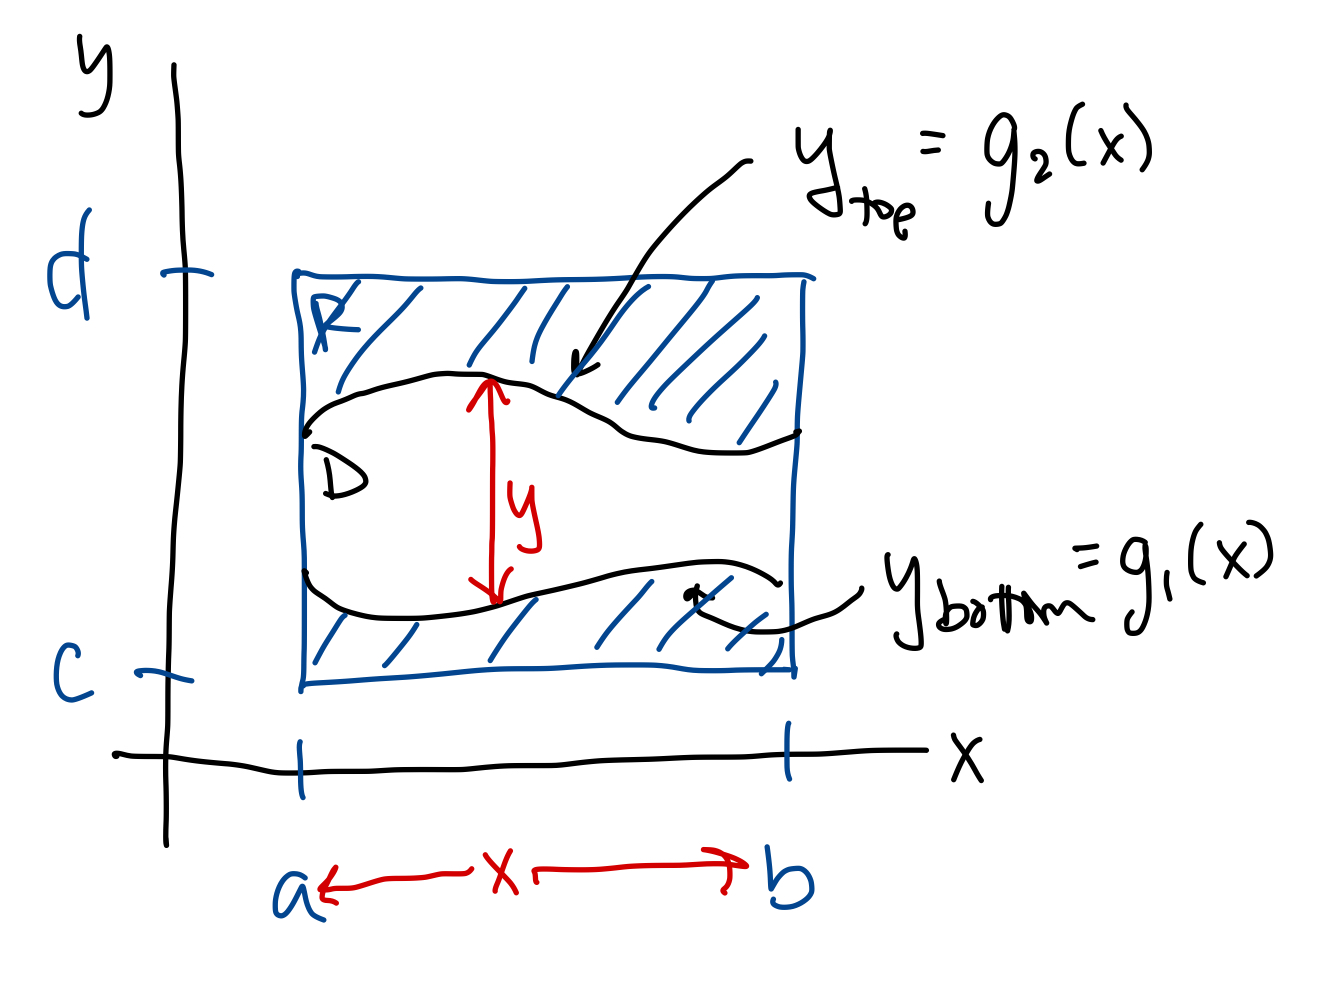
\includegraphics[height=2in]{Ch12s2-TypeI.jpeg}

\[
\iint_D f(x,y)\ dA = \int_a^b \int_{g_1(x)}^{g_2(x)} f(x,y)\ dy\ dx
\]

%\columnbreak

\section*{Horizontally Simple or Type II Regions:}

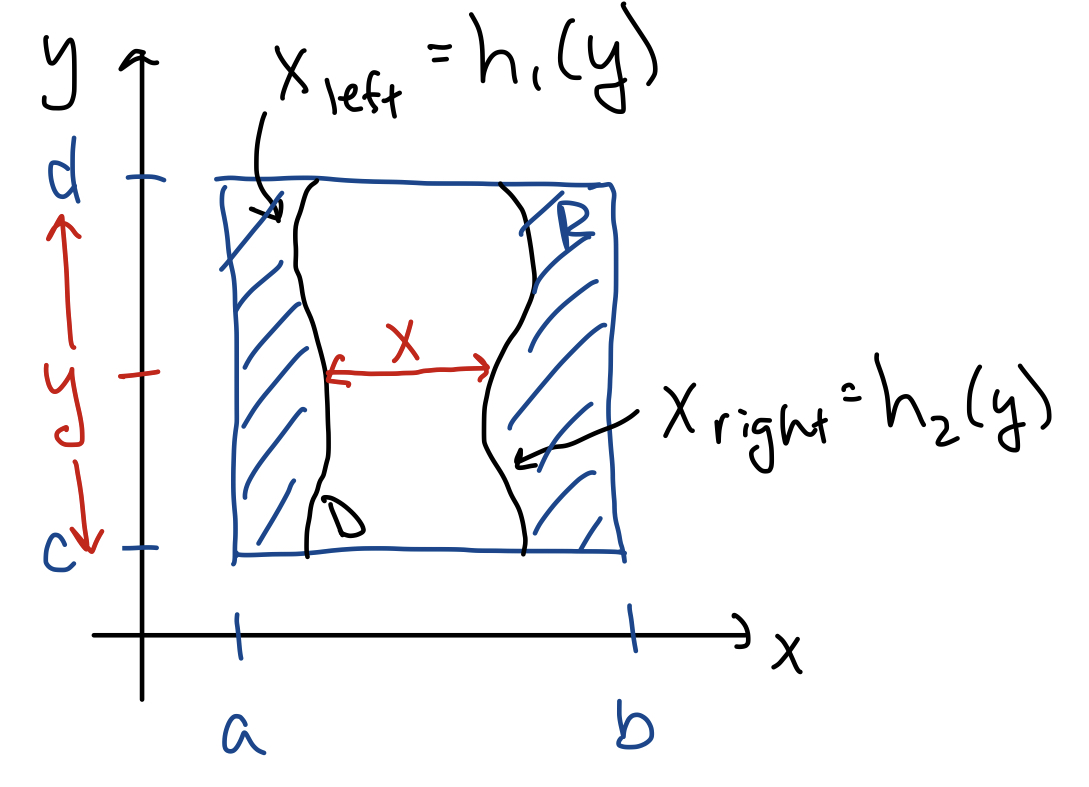
\includegraphics[height=2in]{Ch12s2-TypeII.jpeg}

\[
\iint_D f(x,y)\ dA = \int_c^d \int_{h_1(y)}^{h_2(y)} f(x,y)\ dx\ dy
\]




%\end{multicols}
%
%\end{framed}
%
%\end{minipage}

%\section*{Warm-Up: Type I, TypeII, Neither, or Both?}
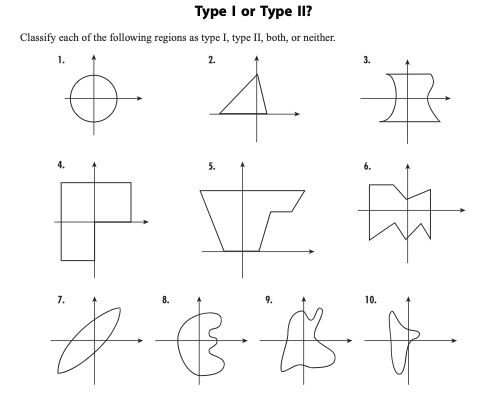
\includegraphics[width=.9\textwidth]{TypeI-or-TypeII.png}

\section*{Examples:}


\begin{enumerate}[{Example} 1: ]
\item Find the volume of the region under \(f(x,y) = 4x+10y\) above the region \(D\) in the \(xy-\)plane that is bounded below by \(y=x\) and above by \(y=x^2\), to the left by \(x=1\) and to the right by \(x=2\).

\vfill

\item Evaluate \(\iint_{D} x^2+y^2\ dA\) where \({D}\) is the region in the \(xy-\)plane bounded by \(x=y\) and \(x=y^2\).

\vfill

\item Evaluate \(\int_0^1 \int_x^1 e^{y^2}\ dy\ dx\).

\vfill

\item Evaluate \(\iint_{D} x+y\ dA\) for the region \(D\) shaded below.

\begin{minipage}{.3\textwidth}
%\hspace*{-.5in}
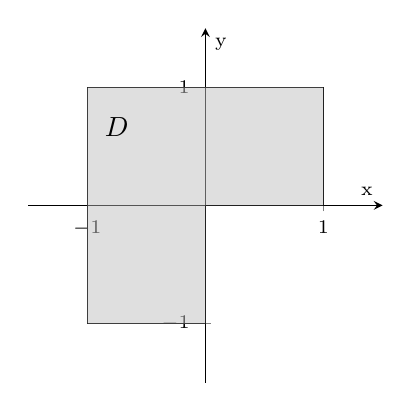
\begin{tikzpicture}
\begin{axis}[
	y=1.5cm,
    x=1.5cm,
	axis x line=middle,
	axis y line = middle,
	xmin=-1.5,xmax=1.5,
	ymin=-1.5,ymax=1.5,
    grid=none,
    %ticks=none,
%    xticklabels={0,$\frac{\pi}{4}$,$\frac{\pi}{2}$},
%    yticklabels={0,1},
    xtick={-1,1},
    ytick={-1,1},
%    yticklabels={0,1},
    xlabel=x,
    ylabel=y,
    label style={font=\scriptsize},
    tick label style={font=\scriptsize},
%    stack plots=y,
    samples=100
]


%\addplot+[name path=A,black,domain=0:1.57, samples=100, smooth] {cos(deg(x))};
%\addplot+[name path=B,black,domain=0:1.57, samples=100, smooth] {sin(deg(x))};
%
%\addplot[blue!50,domain:0,.785] fill between[of=A and B];

\addplot+[black,mark=none, domain=-1:1, smooth]{1};   
\addplot+[black,mark=none, domain=-1:0, smooth]{-1};   
\addplot+[black,mark=none, domain=-1:1, smooth](-1,x);   
\addplot+[black,mark=none, domain=0:1, smooth](1,x);      
\addplot[fill=gray!50,
    fill opacity=0.5,domain=-1:1,draw=none]{1}   
       \closedcycle;
\addplot[fill=gray!50,
    fill opacity=0.5,domain=-1:0,draw=none]{-1}   
       \closedcycle;


%\addplot +[blue, thick, mark=none, domain=0:1.57, samples=100, smooth] {cos(deg(x))};
%\addplot +[blue, thick, mark=none, domain=0:1.57, samples=100, smooth] {sin(deg(x))};

\node [above] at (axis cs:  -.75,.5) {$D$};

%\node [right] at (axis cs: 3,3) {{\tiny $(3,3)$}};


\end{axis}
\end{tikzpicture}
\end{minipage}



\end{enumerate}

\pagebreak

\section*{Group Work:}

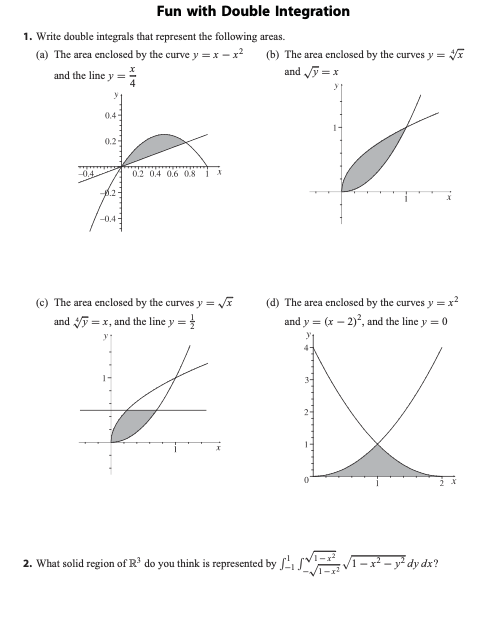
\includegraphics[height=.9\textheight]{Fun-with-Double-Integration.png}

\end{document}

